\chapter{Systemarkitektur}

Dette afsnit præsenterer systemets arkitektur i en grad der gør det muligt at forstå sammensætningen mellem dets hardware og software komponenter.

\section{Domænemodel}

På figur \ref{figure:domainModel} ses domænemodellen af systemet. Denne har til formål at præsentere forbindelserne mellem systemets komponenter, samt dets grænseflader.

\begin{figure}[H]
	\centering
	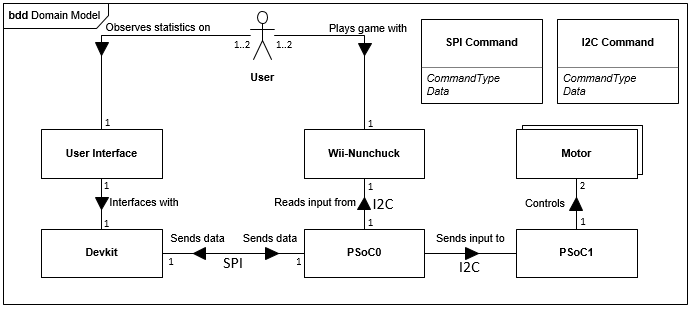
\includegraphics[width=\textwidth]{SystemArkitektur/images/DomainModel.PNG}
	\caption{Systemets domænemodel}
	\label{figure:domainModel}
\end{figure}

Her repræsenteres hardware som blokke forbundet med associeringer. Associeringerne viser grænsefladerne mellem de forbundne hardware komponenter (Enten \textit{SPI} eller \textit{I2C}), samt retningen af kommunikationen. Af modellen fremstår konceptuelle kommandoer for grænsefladerne, som beskriver deres nødvændige attributter.

\section{Software Allokering}

Domænemodellen i figur \ref{figure:allocationDiagram} præsenterer systemets hardwareblokke. På figur \ref{figure:allocationDiagram} ses et software allokeringsdiagram, som viser hvilke hardwareblokke der har softwaredele af systemet allokeret på sig. 

\begin{figure}[H]
	\centering
	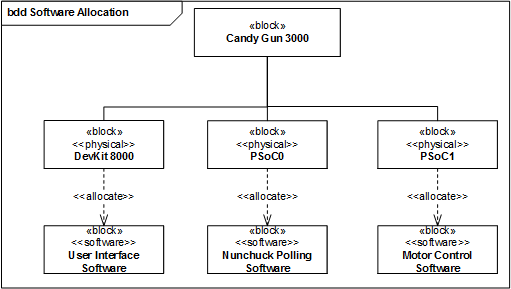
\includegraphics[width=\textwidth]{SystemArkitektur/images/SoftwareAllocation.PNG}
	\caption{Systemets software allokeringer}
	\label{figure:allocationDiagram}
\end{figure}

Det kan her ses at systemet består af tre primære softwaredele: \textit{User Interface Software}, \textit{Nunchuck Polling Software}, \textit{Motor Control Software}. Disse er fordelt over de tre viste CPU'er.

På figurerne: \ref{fig:UserInterfaceAllocationClasses}, \ref{fig:NunchuckPollingAllocationClasses}, \ref{fig:MotorControlAllocationClasses} ses et overblik over konceptuelle klasser der repræsenterer ansvarsområder de primære softwaredele får. For en beskrivelse af design og implementering af disse primære softwaredele henvises til \textbf{DESIGN OG IMPLEMENTERING \#ref}.

På figur \ref{fig:UserInterfaceAllocationClasses} ses det at \textit{User Interface Software}, allokeret på DevKit 8000, har ansvar for brugergrænsefladen samt en SPI Driver til kommunikation med PSoC0. 

\begin{figure}[H]
	\centering
	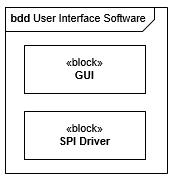
\includegraphics[width=0.4\textwidth]{SystemArkitektur/images/UserInterfaceAllocationClasses.PNG}
	\caption{Systemets software allokeringer}
	\label{fig:UserInterfaceAllocationClasses}
\end{figure}

På figur \ref{fig:NunchuckPollingAllocationClasses} ses det at \textit{Nunchuck Polling Software}, allokeret på PSoC0, har ansvar for en I2C Driver, SPI Driver, samt en Nunchuck API. I2C Driveren skal bruges til kommunikation med den fysiske Nunchuck controller samt PSoC1. SPI Driveren skal bruges til kommunikation med DevKit 8000. Nunchuck API'en bruges for at tilgå data'en fra den fysiske Nunchuck controller.

\begin{figure}[H]
	\centering
	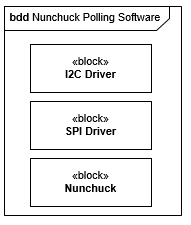
\includegraphics[width=0.4\textwidth]{SystemArkitektur/images/NunchukPollingAllocationClasses.PNG}
	\caption{Systemets software allokeringer}
	\label{fig:NunchuckPollingAllocationClasses}
\end{figure}

På figur \ref{fig:MotorControlAllocationClasses} ses det at \textit{Motor Control Software}, allokeret på PSoC1, har ansvar for en I2C Driver til kommunikation med PSoC0, samt en Motor Driver til motorstyring.

\begin{figure}[H]
	\centering
	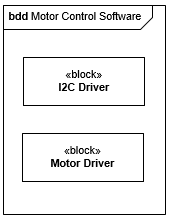
\includegraphics[width=0.4\textwidth]{SystemArkitektur/images/MotorControlAllocationClasses.PNG}
	\caption{Systemets software allokeringer}
	\label{fig:MotorControlAllocationClasses}
\end{figure}

\section{Hardware}

\subsection{BDD}
\label{afsnit:BDD}
På figur \ref{figure:bddDiagram} ses BDD'et for systemet.

\begin{figure}[H]
	\centering
	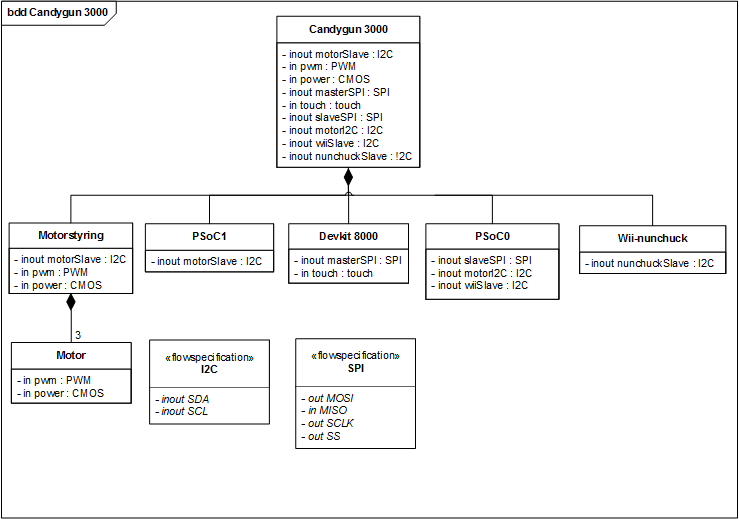
\includegraphics[width=\textwidth]{SystemArkitektur/images/BDD_overordnet.PNG}
	\caption{BDD af systemets hardware}
	\label{figure:bddDiagram}
\end{figure}

Her vises alle hardwareblokke fra domænemodellen (figur \ref{figure:domainModel}) med nødvændige indgange og udgange for de fysiske signaler. Yderligere ses det at flow specifikationer er defineret for de ikke-atomare forbindelser \textit{I2C} samt \textit{SPI}, da disse er busser bestående af flere forbindelser. Der henvises til \textbf{IBD AFSNIT} for en detaljeret model af de fysiske forbindelser mellem hardwareblokkende.

\subsection{Blokbeskrivelse}
Følgende afsnit indeholder en blokbeskrivelse samt en flowspecifikation for I2C og SPI. I flowspecifikationen beskrives I2C og SPI forbindelserne mere detaljeret fra en masters synsvinkel. \newline

\noindent \textbf{DevKit 8000} \par
\noindent \textit{DevKit 8000} er en embedded Linux platform med touch-skærm, der bruges til brugergrænsefladen for produktet. Brugeren interagerer med systemet og ser status for spillet via Devkit 8000. 

\noindent \textbf{Wii-Nunchuck} \par
\noindent \textit{Wii-Nunchuck} er controlleren som brugeren styrer kanonens retning med.

\noindent \textbf{PSoC0} \par
\noindent \textit{PSoC0} er PSoC hardware der indeholder software til I2C og SPI kommunikationen og afkodning af Wii-Nunchuck data. PSoC0 fungerer som I2C master og SPI slave. Denne PSoC er bindeleddet mellem brugergrænsefladen og resten af systemets hardware.

\noindent \textbf{Motor} \par
\noindent \textit{Motor} blokken er Candy Gun 3000's motorerer, der anvendes til at bevæge kanonen i forskellige retninger.

\noindent \textbf{PSoC1} \par
\noindent \textit{PSoC1} er PSoC hardware der indeholder software til I2C kommunikatioon og styring af Candy Gun 3000's motorer. PSoC1 fungerer som I2C slave.


\noindent \textbf{SPI (FlowSpecification)} \par
\noindent \textit{SPI (FlowSpecification)} beskriver signalerne der indgår i \textit{SPI} kommunikation.

\noindent \textbf{I2C (FlowSpecification)} \par
\noindent \textit{I2C (FlowSpecification)} beskriver signalerne der indgår i \textit{I2C} kommunikation.

\subsection{IBD}
\label{afsnit:IBD}

På figur \ref{figure:ibdDiagram} ses IBD'et for systemet.

\begin{figure}[H]
	\centering
	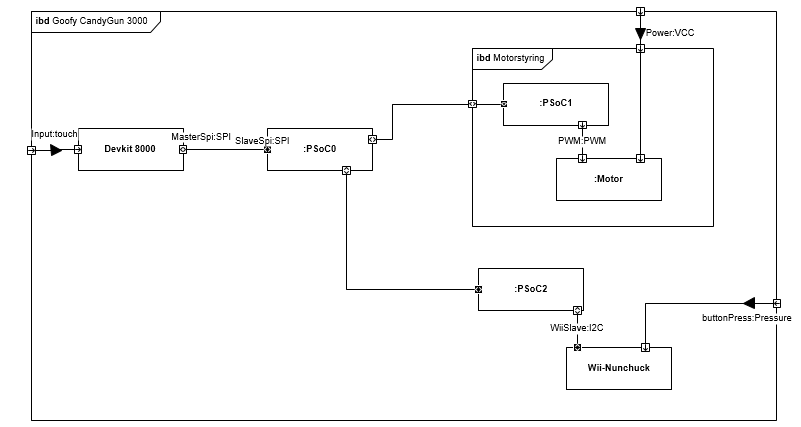
\includegraphics[width=\textwidth]{SystemArkitektur/images/GoofyCandyIBDImageRev2.PNG}
	\caption{IBD af systemets hardware}
	\label{figure:ibdDiagram}
\end{figure}

Her vises alle hardwareblokke med de fysiske forbindelser beskrevet i BDD'et (figur \ref{figure:bddDiagram}). 

Det ses at systemet bliver påvirket af tre eksterne signaler: \textit{touch}, \textit{input}, samt \textit{voltage}. \textit{touch} er input fra brugeren når der interageres med brugergrænsefladen. \textit{input} er brugerens interaktion med Wii-Nunchuk. \textit{voltage} er forsyningsspænding til systemet.

\subsection{Signalbeskrivelse}
\begin{longtable}{|>{\hspace{0pt}}p{3cm} | >{\hspace{0pt}}p{3cm} | p{2cm} | p{3cm} |}
	\hline
	\textbf{Blok-navn} & \textbf{Funktionsbeskrivelse} & \textbf{Signaler} & \textbf{Signalbeskrivelse} \\ \hline
	Devkit 8000 & Fungerer som grænseflade mellem bruger og systemet samt SPI master. & masterSPI & Type: SPI \newline Spændingsniveau: 0-5V \newline Hastighed: ?? \newline Beskrivelse: SPI bussen hvori der sendes og modtages data.\\ \cline{3-4}
	& & touch & Type: touch \newline Beskrivelse: Brugertryk på Devkit 8000 touchdisplay. \\ \hline
	PSoC0 & Fungerer som I2C master for PSoC1 og Wii-Nunchuck samt SPI slave til Devkit 8000. & slaveSPI & Type: SPI \newline Spændingsniveau: 0-5V \newline Hastighed: ?? \newline Beskrivelse: SPI bussen hvori der sendes og modtages data.\\ \cline{3-4}
	& & wiiMaster & Type: I2C \newline Spændingsniveau: ?? \newline Hastighed: ?? \newline Beskrivelse: I2C bussen hvor der modtages data fra Nunchuck.\\ \cline{3-4}
	& & motorMaster & Type: I2C \newline Spændingsniveau: 0-5V \newline Hastighed: 100kbit/sekund \newline Beskrivelse: I2C bussen hvor der sendes afkodet Nunchuck data til PSoC1.\\ \hline
	PSoC1 & Modtager nunchuckinput fra PSoC0 og omsætter dataene til PWM signaler. & motorSlave & Type: I2C \newline Spændingsniveau: 0-5V \newline Hastighed: 100kbit/sekund \newline Beskrivelse: Indeholder formatteret Wii-Nunchuck data som omsættes til PWM-signal. \\ \cline{3-4} 
	& & PWM & Type: PWM \newline Frekvens: 22kHz \newline PWM \%: 0-100\% \newline Spændingsniveau: 0-5V \newline Beskrivelse: PWM signal til styring af motorens hastighed. \\ \hline
	Motor & Den enhed der skal bevæge kanonen & PWM & Type: PWM \newline Frekvens: 22kHz \newline PWM\%: 0-100\% \newline Spædingsniveau: 0-5V \newline Beskrivelse: PWM signal til styring af motorens hastighed. \\ \cline{3-4}
	& & motorVoltage & Type: voltage \newline Spændingsniveau: 12V \newline Beskrivelse: Strømforsyning til motoren \\ \hline
	Wii-nunchuck & Den fysiske controller som brugeren styrer kanonen med. & wiiSlave & Type: I2C \newline Spændingsniveau: 0-5V \newline Hastighed: 100kbit/sekund \newline Beskrivelse: Kommunikationslinje mellem PSoC1 og Wii-Nunchuck. \\ \cline{3-4}
	& & userInput & Type: input \newline Beskrivelse: Brugerinput fra Wii-Nunchuck. \\ \hline
	SPI & Denne blok beskriver den ikke-atomiske SPI forbindelse. & MOSI & Type: CMOS \newline Spændingsniveau: 0-5V \newline Hastighed: ?? \newline Beskrivelse: Binært data der sendes fra master til slave. \\ \cline{3-4}
	& & MISO & Type: CMOS \newline Spændingsniveau: 0-5V \newline Hastighed: ?? \newline Beskrivelse: Binært data der sendes fra slave til master. \\ \cline{3-4}
	& & SCLK & Type: CMOS \newline Spændingsniveau: 0-5V \newline Hastighed: ?? \newline Beskrivelse: Clock signalet fra master til slave, som bruges til at synkronisere den serielle kommunikation. \\ \cline{3-4}
	& & SS & Type: CMOS \newline Spændingsniveau: 0-5V \newline Hastighed: ?? \newline  Beskrivelse: Slave-Select, som bruges til at bestemme hvilken slave der skal kommunikeres med. \\ \hline
	I2C & Denne blok beskriver den ikke-atomiske I2C forbindelse. & SDA & Type: CMOS \newline Spændingsniveau: 0-5V \newline Hastighed: ?? \newline Beskrivelse: Databussen mellem I2C masteren og I2C slaver. \\ \cline{3-4}
	& & SCL & Type: CMOS \newline Spændingsniveau: 0-5V \newline Hastighed: ?? \newline Beskrivelse: Clock signalet fra master til lyttende I2C slaver, som bruges til at synkronisere den serielle kommunikation. \\ \hline
	\caption{Tabel med signalbeskrivelse}
\end{longtable}


\section{Software}

\subsection{SPI Kommunikations Protokol}
I afsnittet \ref{afsnit:IBD} \textbf{IBD} ses det på IBD'et (figur \ref{figure:ibdDiagram}) at Devkit8000 og PSoC0 kommunikerer med hinanden via en SPI bus. Kommunikationen foregår ved at der sendes kommandotyper imellem de to enheder. På tabel \ref{tabel:spiKommandoType} ses en tabel over de brugte kommandotyper og en kort beskrivelse for hver af disse.

\begin{table}[H]
	\centering
	\resizebox{\textwidth}{!}{%
		\begin{tabular}{llll}
			\hline
			\multicolumn{1}{|l|}{Kommandotype}                                & \multicolumn{1}{l|}{Beskrivelse}                        & \multicolumn{1}{l|}{Binær Værdi} & \multicolumn{1}{l|}{Hex Værdi} \\ \hline
			\rowcolor[HTML]{CBCEFB} 
			{\color[HTML]{000000} START\_SPI\_TEST}                           & {\color[HTML]{000000} Sætter PSoC0 i 'SPI-TEST' mode}   & 1111 0001                        & 0xF1                           \\
			START\_I2C\_TEST                                                  & Sætter PSoC0 i 'I2C-TEST' mode                          & 1111 0010                        & 0xF2                           \\
			\rowcolor[HTML]{CBCEFB} 
			\begin{tabular}[c]{@{}l@{}}START\_NUN-\\ CHUCK\_TEST\end{tabular} & Sætter PSoC0 i 'NUNCHUCK-TEST' mode                     & 1111 0011                        & 0xF3                           \\
			SPI\_OK                                                           & Signalerer at SPI-testen blev gennemført uden fejl      & 1101 0001                        & 0xD1                           \\
			\rowcolor[HTML]{CBCEFB} 
			I2C\_OK                                                           & Signalerer at I2C-testen blev gennemført uden fejl      & 1101 0010                        & 0xD2                           \\
			I2C\_FAIL                                                         & Signalerer at der skete fejl under I2C-testen           & 1100 0010                        & 0xC2                           \\
			\rowcolor[HTML]{CBCEFB} 
			NUNCHUCK\_OK                                                      & Signalerer at NUNCHUCK-testen blev gennemført uden fejl & 1101 0011                        & 0xD3                           \\
			NUNCHUCK\_FAIL                                                    & Signalerer at der skete fejl under NUNCHUCK-testen      & 1100 0011                        & 0xC3                          
		\end{tabular}
	}
	\caption{Kommandotyper der anvendes ved SPI kommunikation}
	\label{tabel:spiKommandoType}
\end{table}


\subsection{I2C Kommunikations Protokol}

I afsnittet \ref{afsnit:IBD} \textbf{IBD} ses det på IBD'et (figur \ref{figure:ibdDiagram}) at tre hardwareblokke kommunikerer med hinanden via en I2C bus. Til denne I2C kommunikation er der defineret en protokol, som sætter en standard for hvordan modtaget data skal fortolkes. Denne protokol beskrives her.

I2C gør brug af en indbygget protokol der anvender adressering af hardware-enheder for at identificere hvilken enhed der kommunikeres med. Derfor har hardwareblokkene som indgår i I2C kommunikation fået tildelt adresser. På tabel \ref{table:I2CAddress} ses adresserne tildelt systemets PSoCs.

\begin{table}[H]
	\centering
	\begin{tabular}{llllllllll}
		\hline
		\multicolumn{1}{|l|}{I2C Adresse bits} & 7                        & 6                        & 5                        & 4 & 3 & 2 & \multicolumn{1}{l|}{1} & \multicolumn{1}{l|}{0 (R/W)} \\ \hline
		\rowcolor[HTML]{CBCEFB} 
		{\color[HTML]{000000} PSoC0}           & {\color[HTML]{000000} 0} & {\color[HTML]{000000} 0} & {\color[HTML]{000000} 0} & 1 & 0 & 0 & 0                      & 0/1                          \\
		PSoC1                                  & 0                        & 0                        & 0                        & 1 & 0 & 0 & 1                      & 0/1 \\
		\rowcolor[HTML]{CBCEFB} 
		{\color[HTML]{000000} Wii-Nunchuck}           & {\color[HTML]{000000} 1} & {\color[HTML]{000000} 0} & {\color[HTML]{000000} 1} & 0 & 0 & 1 & 0                      & 0/1                      
	\end{tabular}
	\caption{Adresser der anvendes på I2C bussen}
	\label{table:I2CAddress}
\end{table}

Da I2C dataudveksling sker bytevist, er kommunikations protokollen opbygget ved, at kommandoens type indikeres af den første modtagne byte. Herefter følger \textit{N}-antal bytes som er kommandoens tilhørende data. \textit{N} er et vilkårligt heltal og bruges i dette afsnit når der refereres til en mængde data-bytes der sendes med en kommandotype.

Kommandoens type definerer antallet af databytes modtageren skal forvente og hvordan disse skal fortolkes. På figur \ref{fig:I2CProtokolEksempel} ses et sekvensdiagram der, med pseudo-kommandoer, demonstrerer forløbet mellem en I2C afsender og modtager ved brug af kommunikations protokollen.

\begin{figure}[H]
	\centering
	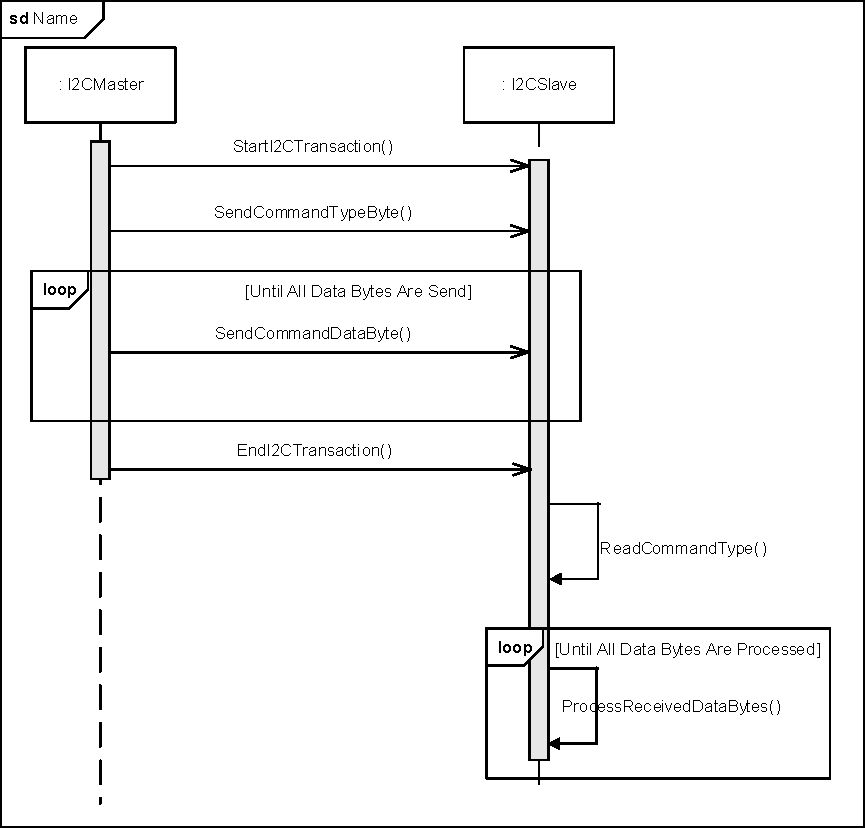
\includegraphics[width=\textwidth] {Systemarkitektur/images/I2CProtocol}
	\caption{Eksempel af I2C Protokol Forløb}
	\label{fig:I2CProtokolEksempel}
\end{figure}

På figur \ref{fig:I2CProtokolEksempel} ses at afsenderen først starter en I2C transaktion, hvorefter typen af kommando sendes som den første byte. Efterfølgende sendes \textit{N} antal bytes, afhængig af hvor meget data den givne kommandotype har brug for at sende. Efter afsluttet I2C transaktion læser I2C modtageren typen af kommando, hvor den herefter kan fortolke \textit{N} antal modtagne bytes afhængig af den modtagne kommandotype.

På tabel \ref{table:I2CKommandoer} ses de definerede kommandotyper og det tilsvarende antal af bytes der sendes ved dataveksling.

\begin{table}[H]
	\centering
	\resizebox{1.2\textwidth}{!}{
		\begin{tabular}{lllll}
			\hline
			\multicolumn{1}{|l|}{Kommandotype}    & \multicolumn{1}{l|}{Beskrivelse}                                            & \multicolumn{1}{l|}{Binær Værdi} & \multicolumn{1}{l|}{Hex Værdi} & \multicolumn{1}{l|}{Data Bytes}                                                                                         \\ \hline
			\rowcolor[HTML]{CBCEFB} 
			{\color[HTML]{000000} NunchchuckData} & {\color[HTML]{000000} Indeholder aflæst data fra Wii Nunchuck controlleren} & 0010 1010                        & 0xA2                           & \begin{tabular}[c]{@{}l@{}}Byte \#1 Analog X-værdi\\ Byte \#2 Analog Y-værdi\\ Byte \#3 Analog Buttonstate\end{tabular} \\
			I2CTestRequest                        & Anmoder PSoC0 om at starte I2C-kommunikations test                          & 0010 1001                        & 0x29                           & Ingen databyte                                                                                                          \\
			\rowcolor[HTML]{CBCEFB} 
			I2CTestAck                            & Anmodning om at få en I2C OK besked fra I2C enhed                           & 0010 1000                        & 0x28                           & Ingen databyte                                                                                                         
		\end{tabular}
	}
	\caption{Kommandotyper der anvendes ved I2C kommunikation}
	\label{table:I2CKommandoer}
\end{table}

Kolonnerne "Binær Værdi" og "Hex Værdi" i tabel \ref{table:I2CKommandoer} viser kommandotypens unikke tal-ID i både binær- og hexadecimalform. Denne værdi sendes som den første byte, for at identificere kommandotypen. 

\subsection{Specifikation og Analyse}